% This Labbook describes the development of mismatch models of CORN
% Zheng Hu and Sherry Dongqi Bao
% Created July 2018
% Last change July 2018



\documentclass[a4paper,10pt]{article}


\usepackage{lineno,hyperref}
\usepackage[utf8]{inputenc}
\usepackage{bm}
\usepackage{amsmath}
\usepackage{amssymb}
\usepackage{amssymb}
\usepackage[pdftex]{graphicx}
\usepackage{xcolor}
\definecolor{darkblue}{rgb}{0,0,0.5}
\usepackage{transparent}
\usepackage{algpseudocode}
\usepackage{algorithm}
\usepackage{hyperref}
\usepackage{graphicx}
\usepackage{subcaption}
\usepackage{pdfpages}
\usepackage{float} % added to avoid table movement
\usepackage{indentfirst} % added to indent first paragraph

\usepackage[backend=bibtex, style=numeric, sorting=none]{biblatex}
\usepackage{csquotes}
\addbibresource{reference.bib}

\usepackage{titlesec}
\setcounter{secnumdepth}{4}
\titleformat{\paragraph}
{\normalfont\normalsize\bfseries}{\theparagraph}{1em}{}
\titlespacing*{\paragraph}
{0pt}{3.25ex plus 1ex minus .2ex}{1.5ex plus .2ex}


\graphicspath{ {Figures/} }
\newcommand{\red}[1]{\textcolor{red}{#1}}
\newcommand{\green}[1]{\textcolor{green}{#1}}
\newcommand{\magenta}[1]{\textcolor{magenta}{#1}}
\renewcommand*\rmdefault{iwona}
%openings
\DeclareMathOperator*{\argmax}{arg\,max}

\title{Construction of Free Energy Model}
\author{Zheng Hu, Sherry Dongqi Bao \\ Tianjin University}

\begin{document}
\maketitle	
	
\section{Background}
The current models of the off-target problem in the CRISPR-Cas system can be divided into three types. Firstly, it can be modeled as purely "sequence alignment problem" similar to BLAST, which doesn't consider either the energy change or the experiment data; Secondly, it can be modeled with the help of experiment data; Thirdly, in a kinetic model, the energy change will be considered. 

Our model aims to investigate the off-target problem in the CRISPR-Cas system in an innovative kinetic model, therefore finding efficient ways to enhance the reliability of gene editing. Our motivation is based on our project Cell-free cancer detection. Firstly, there are no existing tools for evaluating sgRNA candidates' off-target probability with Cas13a, and the current tool for Cas12a is BLAST-based, which means that it is a rough model and can hardly take the case of single nucleotide mutation of cancer into account. The foundations of our model are mostly simple probability theory and energy theory, which make our model both convincing and pellucid.

\section{Introduction}
Currently, people have constructed a similar model as illustrated in the following figure \ref{fig:1}. There are four common rules when Cas nuclease cleaves the DNA\cite{klein2018hybridization}.
	.
\begin{figure}[tbph]
\centering
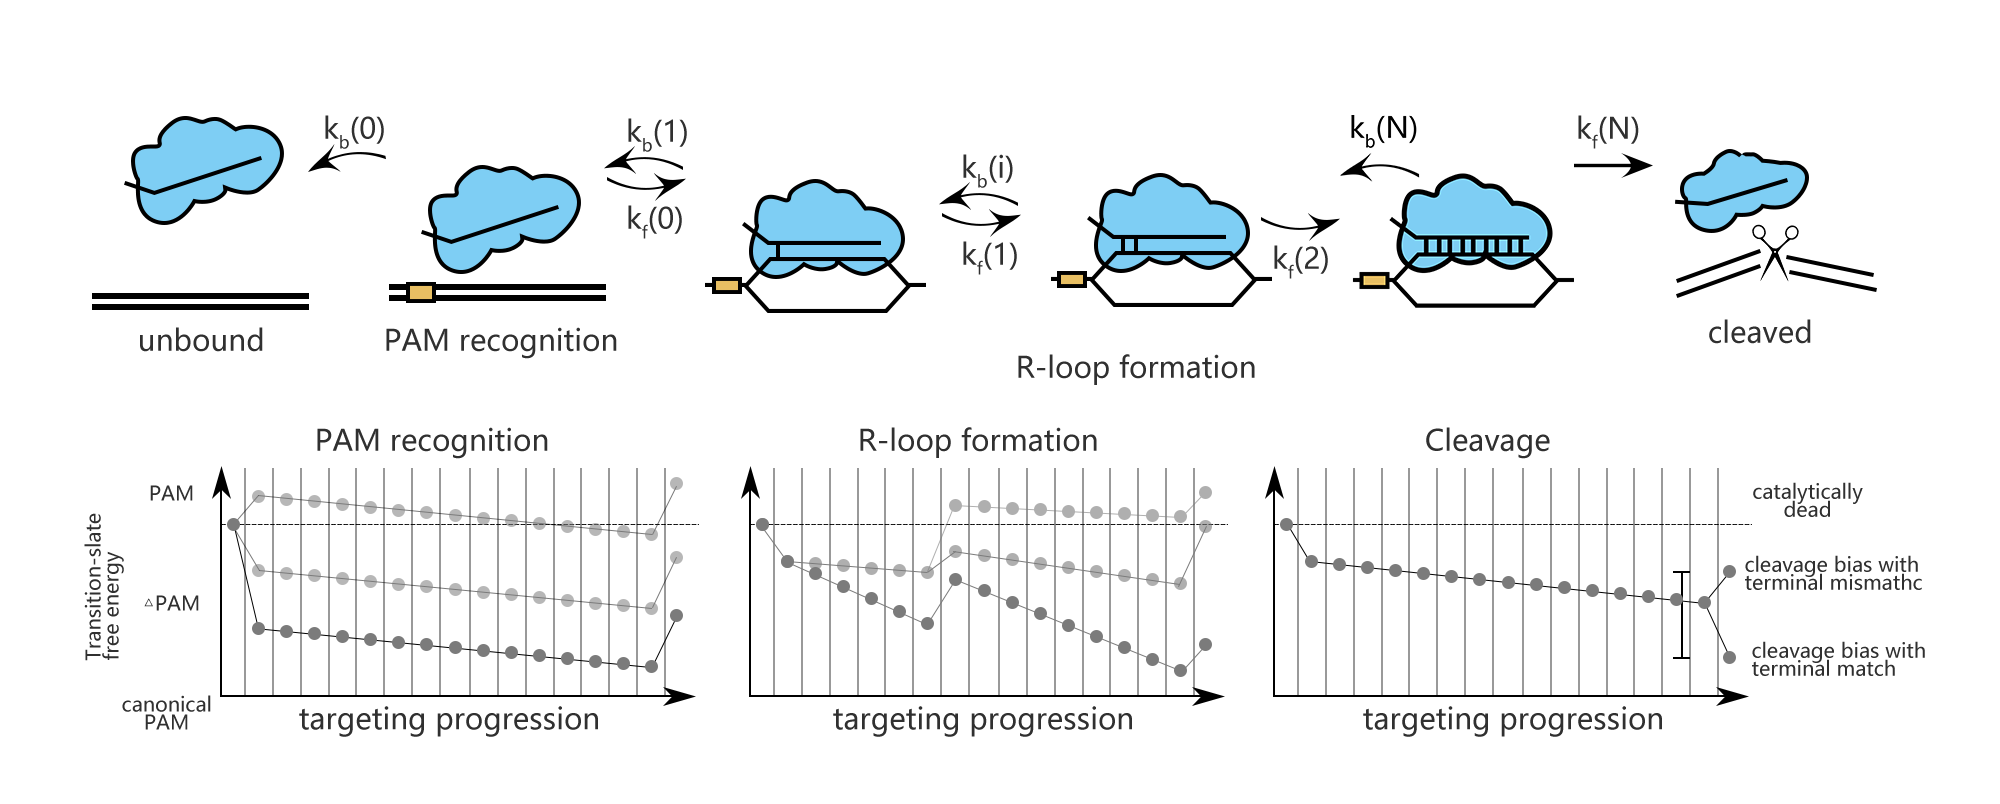
\includegraphics[width=3.5in]{1}
\caption{schematic diagram}
\label{fig:1}
\end{figure}
	
(1) Seed region: single mismatches within a PAM proximal seed region can completely disrupt interference;\par
(2) Mismatch spread: when mismatches are outside the seed region, off-targets with spread-out mismatches are targeted most strongly;\par
(3) Differential binding versus differential cleavage: binding is more tolerant of mismatches than cleavage;\par 
(4) Specificity-efficiency decoupling: weakened protein-DNA interactions can improve target selectivity while still maintaining efficiency;\par

Based on these four rules, probability theory is applied in to explain it. As we know, there are always two results in an experiment, which are successful cleavage and unsuccessful cleavage. In math view, it can be one-hot encoded, and they are corresponding to 1 and 0. 

However, giving a 0/1 prediction is hard and unreliable. To solve this problem, one choice is to consider it as a cluster problem; however, it is easier to find a continuous quantitative function rather than to find a suitable cluster distance function. So naturally, finding an approximate probability distribution is a good choice. 
	
Many current off-target evaluating websites use a score function to evaluate whether the target is good or bad. Here we consider the score function has the similar ability to probability, which is a description of "better" or "worse" while it can’t guarantee whether successful cleavage will appear. For our case, our goal is to find a function indicating which target is BETTER.
	
Considering the difference between model prediction and experimental data, our model consists of two aspects, which are kinetic model and  parameter updating module.
\section{Methods}
\subsection{Kinetic model}
The whole binding-cleavage process begins with the binding between PAM and protein. It corresponds to rule\#1 mentioned before. And as the reaction proceeds, every step of it is reversible, and its irreversibility mainly depends on the binding energy of two DNA bases.
	
Here we use the term binding probability $P_{bind}$ represent the probability of sgRNA binding with DNA, with a rough assumption that the probability of cleavage is the same for every kind of binding. In total, the probability of off-target cleavage is positively correlated with the binding probability. 

The probability $P_{bind,N}$ , representing the probability of binding at the Nth position (the last position of sgRNA) of nucleotide base, is given by:
\begin{equation}
P_{bind,N}=\frac{k_f(N)}{k_f(N)+k_b(N)}=\frac{1}{1+\gamma_N} \quad
\end{equation}
where $k$ is the reaction rate constant; $f$ represents the forward reaction; $b$ represents the backward reaction. And 
\begin{equation}
 \gamma_N=\frac{k_b(N)}{k_f(N)}
\end{equation}
So for a the whole sgRNA sequence: 
\begin{equation}
P_{bind} = \frac{1}{1+\sum_{n=1}^N\coprod_{i=1}^n \gamma_i}
\end{equation}
Consider the rate constant $k_f(i)$ and $k_b(i)$:
\begin{equation}
k_f(i)=k_0exp(-(T_{i,i+1}-F_i)),k_b(i)=k_0exp(-(T_{i,i-1}-F_i))
\end{equation}
where $F_i$ means free energy of each metastable state, $T_{i,i+1}$ means the highest free energy point on the reaction path from position i to position i + 1. Therefore, $T_{i,i+1}-F_i$ is the activation energy of forward reaction and $T_{i,i-1}-F_i$ is activation energy of the backward reaction.
\begin{equation}
\Rightarrow \gamma_i=exp(-\Delta_i), \Delta_i=T_{i,i+1}-T_{i,i-1}
\end{equation}
\begin{equation}
\begin{aligned}
\Rightarrow P_{bind} = \frac{1}{1+\sum_{n=1}^N\coprod_{i=1}^n \gamma_i}=\frac{1}{1+\sum_{n=1}^N\coprod_{i=1}^n exp(-\Delta_i)}\\=\frac{1}{1+\sum_{n=1}^N exp(-\sum_{i=1}^n\Delta_i)}
\end{aligned}
\end{equation}
We define $$\Delta T_n=\sum_{i=1}^n\Delta_i$$
so
\begin{equation} 
P_{bind} =\frac{1}{1+\sum_{n=1}^N exp(-\Delta T_n)}
\end{equation}
	
From the above, it is clear that the binding probability depends only on the state transition energy, not on the free energy of metastable states. If we assume there is one dominant bias $\Delta T_{n^*}$, then this equation can be approximated as:
\begin{equation}
 P_{bind} \approx \frac{1}{1+exp(-\Delta T_{n^*})}
\end{equation}

As figure shows, we analyze the energy change of every process:\newline
$\left\{
\begin{tabular}{l}
for the PAM position (i = 0) we have $\Delta_0=\Delta PAM$\\
for a partial R-loop we have $\Delta_i = \Delta_M$ if matched and $\Delta_i = -\Delta_U$ mismatched\\
\end{tabular}
\right.$

\begin{equation}
\Delta {T_n} = {\Delta _{PAM}} + {n_M}{\Delta _M} - (n - {n_M}){\Delta _U} - {\delta _{n,N}}{\Delta _{clv}};\:n = 0...N
\end{equation}
where $n_M$ is the number of matches, $\Delta _{clv}$ is the energy change of cleavage after the process of binding is finished.\\
$\delta_{n,N}$ represents the Kronecker delta:
$\delta_{n,N}$=$\left\{\begin{array}{l}1, n=N;\\
0, n\neq N.
\end{array}
\right.$

For PAM independent systems (such as Cas13a), we instead use:
\begin{equation}
\Delta {T_n} = {n_M}{\Delta _M} - (n - {n_M}){\Delta _U} - {\delta _{n,N}}{\Delta _{clv}};\:n = 0...N
\end{equation}

To sum up, the binding probability mainly relies on the free energy change, and PAM appears as a significant energy decline.

\begin{figure}[H]
	\centering
	\includegraphics[width=0.7\linewidth]{AT}
	\caption{Hydrogen bonds between AT}
	\label{fig:6}
\end{figure}
\begin{figure}[H]
	\centering
	\includegraphics[width=0.7\linewidth]{CG}
	\caption{Hydrogen bonds between CG}
	\label{fig:7}
\end{figure}

The kinetic model sets up a framework to build the relationship between binding probability and the numbers of nucleotide matches and mismatches. In consideration of this problem more carefully, the binding probability becomes equal to the analysis of energy change, because we know the binding energy of A/T and C/G is different due to the different hydrogen bonds between them (figure \ref{fig:6} and \ref{fig:7}), and the energy decrease in C/G is approximately 1.5 folds as A/T. Similarly, the mismatch has more types of variance because the sizes of nucleotides are various. Hence, the types of the mismatched base pair are classified by group volume, i.e., two pyrimidines (such as C/T, “Large”), pyrimidine and purine (such as C/A, “Medium”), two purine (such as G/T, “Small”). Hence, the probability can be calculated using the following equation:
\begin{equation}
P_{bind}=\frac{1}{1+e^{-n_1\Delta_{A/T}-n_2\Delta_{C/G}+n_3\Delta_{L}+n_4\Delta_{M}+n_5\Delta_{S}}}
\end{equation}

\subsection{Parameter Optimization}
From the kinetic model, we can get an output, which is the binding probability. It needs to be noticed that the parameters we choose should make results well discriminated, because in a cleavage experiment, we only have two outcomes, successful(1) and unsuccessful(0). 

To make our predictions from the model more approximate to experiment(facts), we set a regression module and implement parameter optimization. Here, the method we choose is stochastic gradient descent (SGD) and cross entropy. Their principles can be concluded as follows:
\begin{equation}
\theta  = \theta  - \eta {\nabla _\theta }J({x^{(i)}},{y^{(i)}},\theta )
\end{equation}
\begin{equation}
loss = \sum\limits_i {{y_i}\ln {y_i}}
\end{equation}
where $\theta$ means the parameter array and J means the loss function. 

Considering the difficulty in gradient calculation, we substitute the differential term with a difference term to accelerate operating speed.\par
\begin{equation}
\frac{{dy}}{{dx}} \approx \frac{{\Delta y}}{{\Delta x}}{\rm{ = }}\frac{{y(x + \delta x) - y(x)}}{{\delta x}}
\end{equation}

By using this simple method, our model can be more vibrant and more reliable with the ability of updating using newest data.

\subsection{Generating sgRNA Candidates}
Meanwhile, we designed a program to generate all the sgRNA candidates for a target gene, and combined with the previous model, we can compare and rank all the candidates.

The principle of the program  is very simple. We use PAM as the input and collect the arrays with a certain length which contain the same beginning code as PAM.


\section{Results}
Here, we set the parameters as default values and observe its performance. Our default parameters are set based on three simple rule. Firstly, because of the different numbers of hydrogen bonds between A/T and C/G, the energy decrease due to A/T binding are 1.5 times to C/G binding. So the parameter\#1 is 1.5 times parameter\#2. Secondly, it's universally known that big compounds with small distance will have a high energy because of repulsion. The mismatching combination between two nucleotides can be classified into three parts--large, medium and small, and we should set other parameters in the same order of values. Thirdly, we use the parameters from \cite{klein2018hybridization} as reference. In total, we set the parameters default values as [0.06,0.09,0.3,0.6,0.03].

 As the following figure shows, the energy always decreases or has some turning point because of mismatch and is always negative. The yellow line represents complete match. The blue line and the red line are two examples of mismatches at different positions. For example, the red line has a peak due to a mismatch, and in our model, we find that it doesn't make the energy positive. It means that in this reaction process there is some force like "momentum" pushing it to proceed and cross the energy peak. For a off-target examination to every location of all the DNA in a system (a genome), there will also be positive energy result, which is obviously not a feasible solution (will not lead to off-target). This kind of results is omitted in the plot.
\begin{figure}[H]
\centering
\includegraphics[width=0.7\linewidth]{energy_change}
\caption{Energy change of sgRNA candidates binding to DNA}
\label{fig:energychange}
\end{figure}

\begin{figure}[H]
\centering
\includegraphics[width=0.7\linewidth]{fig1}
\caption{The possibility of sgRNA candidates binding to DNA's different locations}
\label{}
\end{figure}

After testing our code's running time, we find its rate can reach approximately $2\times10^8\;base/h$ (under parallel computing in 4 cores).

Besides the default parameters, we hope our model can hit more true data. So after we get the experiment data, we can use the parameter optimization method mentioned before to get more precise parameters. 

\addcontentsline{toc}{chapter}{Bibliography}
\printbibliography

\end{document}